\section{Understanding of cache coherence in single core}

Before we determine and analyze MESIF protocol, there are a few important concept
about read-write memory transaction in both single core or multiple cores. To understand
coherence, suppose that we are executing a single core algorithm $S$ on x86 machine and the task
that is sent to processor is to either read or write value to cache at address $A$ where $A$ is 
an arbitrary hexadecimal number. For reading memory by $S$ algorithm, the task is scheduled by CPU 
with read instruction on address $A$ at local cache. Then, the cache on the core is being searched according to
the read instruction and return the value od address $A$ that is currently stored in the cache line as shown in the
figure \ref{fig:read_single_core}.
\begin{figure}[h]
        \centering
        
\includegraphics[width=1\textwidth,scale=0.5]{read_single_core_coherence.png}
        \caption{\label{fig:read_single_core} Read access on cache line}
\end{figure}

Same thing goes the same way with write access on cache. In order to write data into a cache line in a 
particular core, the task of $S$ is being scheduled on core and CPU performs write instruction to address $A$
specify by algorithm $S$ and finish with callback. But, the value on algorithm $S$ will be not be automatically 
update which the algorithm require another read instruction to the same address to retrieve a value as shown in 
figure \ref{fig:write_single_core}. This is also the reason why writing value to cache takes more CPU cycle than read 
in general on both single core and multiple cores. Overall, the timeline of accessing will be write and read repeatedly. 
In single score, everything seems perfectly fine with the design.
Once we run same algorithm in more than 1 processor, there are a drop on performance on accessing cache and memory which will
be determined in the next section.
\begin{figure}[h]
        \centering
        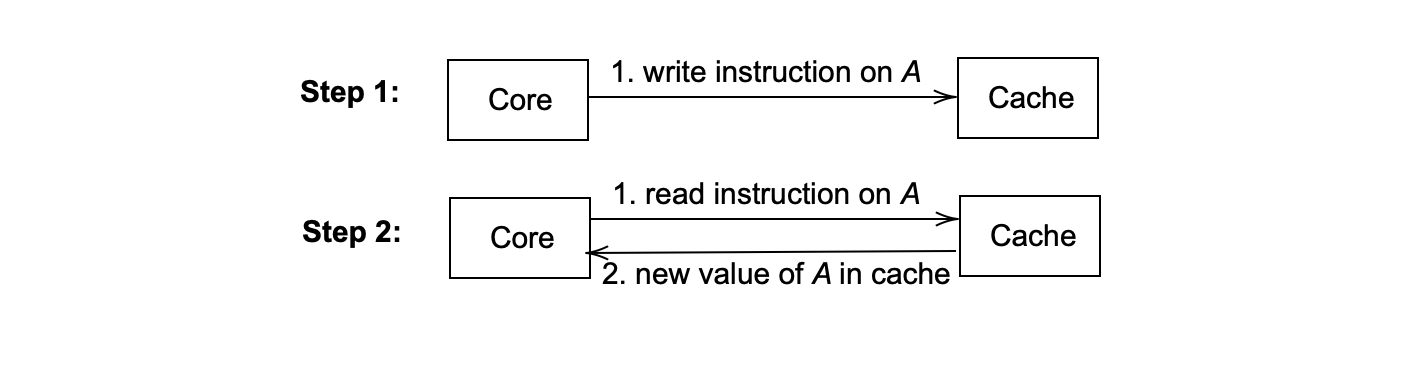
\includegraphics[width=1\textwidth,scale=0.5]{write_single_score_coherence.png}
        \caption{\label{fig:write_single_core} Write access on cache line}
\end{figure}

\section{Understanding of cache coherence in multiple cores}
To understanding coherence when we execute the same algorithm in parallel, suppose that we have 
a program $S$ running on 3 cores $C_1, C_2, C_3$ and accessing the shared memory address $L$.

\begin{figure}[h]
        \centering
        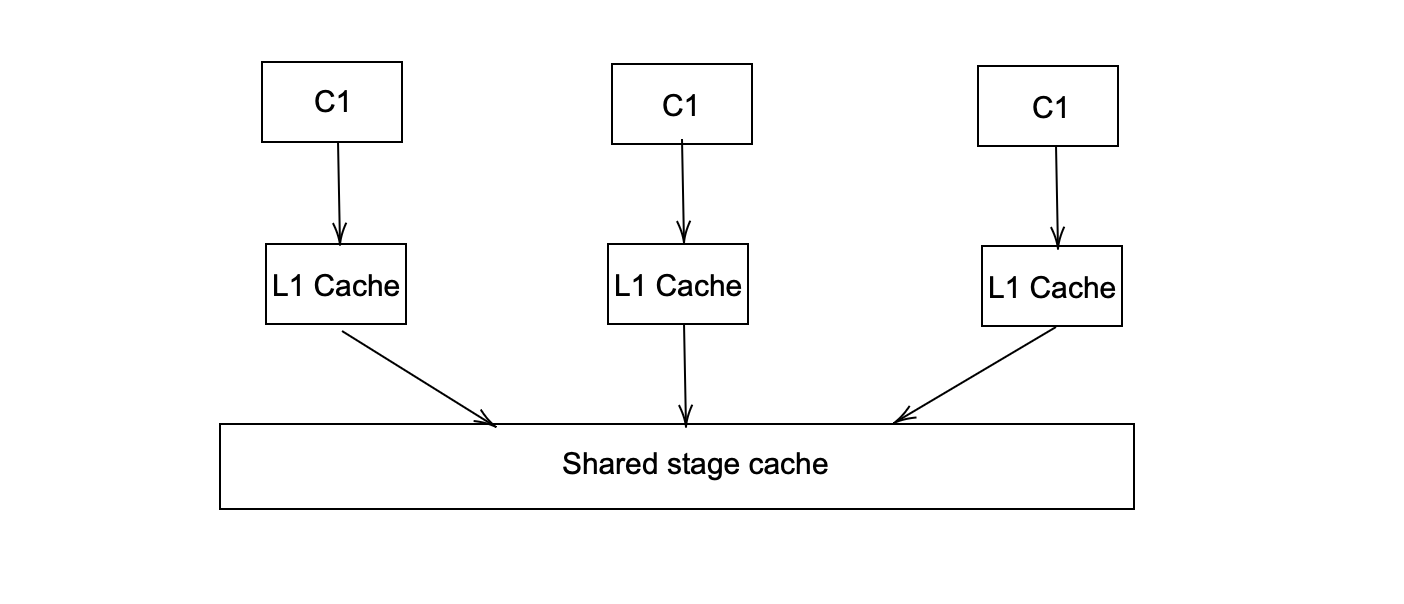
\includegraphics[width=0.7\textwidth,scale=0.5]{multicore_coherence_setup.png}
        \caption{\label{fig:multicore_setup} Parallel access which shared memory}
\end{figure}

Therefore, each core have to read data from address $L$ if their local cache is missing or dirty and some cores
update the value in shared stage memory. The process is similar to single core, but each core needs to communicate
to each other by transferring a message in interconnection network in order to keep the `last' write value to memory.
That means every time core $C_i$ where $i = 1,2,3$ updates the value in memory address $L$ the local cache of the rest 
will become dirty immediately which also means that the core need to inform to others that the value is being updated 
and fetch the value by read instruction. Now the problem begins that decrease the performance. Due to the message delay and latency
between interconnection network, the ordering of write and read disoriented as we need to guarantee that every time we read value
it must be the latest update across all cores. This is also called false sharing. One way to achieve coherency for accesses is to have the writing core wait for all caches
to receive the previous write value before sending a new write task which is called \textbf{an acknowledgement message (ACK)}.

\section{Coherence for Shared Memory in Parallel Execution}
As we explained in the previous section, the concept of coherence in single core applies to all cores when we run tasks
simultaneously on shared memory. A single core executes accesses to a single memory location with an order. When we add caches and multiple cores accessing the same memory locations,
everything does not seem to work out nicely. Caches allow cores to read values written by previous writer and all caches must be updated.
There are two invariants which define what is required for a parallel execution on memory accesses to be consistent which are 
\begin{enumerate}
        \item Single-Write-Multiple-Readers (SWMR): At any time, every memory location $L$  has either one core that may write and read $L$ (writer-reader period), or any number of cores that can only read $L$ (readers period) stated by \cite{hay2012mesif}.
        \item Data-Value: The value of a memory location is the previous value written by this core if this core is writing. Or it is the last value written by the previous writing core, 
                if there is no writer
\end{enumerate}
To clarify more, SWMR invariant guarantees that for each memory location at any time, there is either one writer who can also read location $L$ or many readers who can not write to memory.
The invariant is similar to how rust compiler handle concurrency with ownership. Next, Data-Value invariant states that value of read access
is either the last value written by the previous writing core (the previous writer-reader).

\section{Cache Coherence Protocols}
